\documentclass[conference]{IEEEtran}

\usepackage{cite}
\usepackage{amsmath,amssymb,amsfonts}
\usepackage{algorithmic}
\usepackage{graphicx}
\usepackage{textcomp}
\usepackage{xcolor}
\def\BibTeX{{\rm B\kern-.05em{\sc i\kern-.025em b}\kern-.08em
    T\kern-.1667em\lower.7ex\hbox{E}\kern-.125emX}}
\begin{document}

\title{General Linear Regression of Superconducting Critical Temperature on Superconductor Materials}

\author{\IEEEauthorblockN{Gabriel Guillen}
\IEEEauthorblockA{\textit{dept. of Statistics \& Data Science} \\
\textit{University of Central Florida}\\
Orlando, United States of America \\
ga013701@ucf.edu}}


\maketitle

\begin{abstract}
This paper analyzes the relationship between various material properties and the critical temperature ($T_c$) of superconducting materials. The main objective is to determine if a minimal set of these properties can be used to predict $T_c$ through various general linear models. We will explore several derived metrics and use general linear regression to identify the most significant factors. The findings will demonstrate how these metrics are linearly related to the critical temperature. \\
\end{abstract}

\begin{IEEEkeywords}
Superconductors,
Critical Temperature,
General Linear Model,
Gaussian, Poisson, Tweedie, Predictive Modeling
\end{IEEEkeywords}

\section{\textbf{Introduction}}
This study investigates the linear relationship between a set of predictive metrics and the critical temperature ($T_c$) of various materials. We aim to determine if a linear model can effectively predict $T_c$ and, if so, to identify the most suitable statistical distribution family for this relationship. The data, including several highly correlated derived metrics, will be analyzed to answer these questions. \\
\indent We will begin by detailing the characteristics of the dataset and address any data anomalies. This will be followed by an explanation of the preprocessing methods used to prepare the data for our Generalized Linear Models (GLM). The analysis will incorporate insights from both the training and validation datasets to build and evaluate the predictive models.\\
\indent Finally, we will present which GLM distribution family provides the best fit, as determined by its lowest error rate, for predicting the critical temperature of the materials under consideration.

\section{\textbf{Main Analysis}}

\subsection{\textbf{Data}}

This study utilizes a dataset on superconducting materials, sourced from \cite{hamidieh2018}. The dataset contains information about the chemical composition and critical temperature ($T_c$) for various materials. \\

\subsubsection{\textbf{Data Structure and Features}}

The dataset includes \textbf{eight derived chemical features} for each material's chemical formula:
\begin{itemize}
\item Atomic Mass
\item Atomic Radius
\item Density, Electron Affinity
\item First Ionization Energy (FIE)
\item Fusion Heat
\item Thermal Conductivity
\item Valence
\end{itemize}

\indent These eight features are summarized across \textbf{ten statistical metrics}: \texttt{mean}, weighted mean (\texttt{wtd\_mean}), geometric mean (\texttt{gmean}), weighted geometric mean (\texttt{wtd\_gmean}), \texttt{entropy}, weighted entropy (\texttt{wtd\_entropy}), \texttt{range}, weighted range (\texttt{wtd\_range}), standard deviation (\texttt{std}), and weighted standard deviation (\texttt{wtd\_std}). This results in a total of 80 potential features (8 features × 10 statistical metrics).\\
\indent Additionally, the dataset includes as an additional feature the \textbf{Number of Elements} (\texttt{number\_of\_elements}) in each material's chemical formula. \\

\subsubsection{\textbf{Data Handling}}

The units of measurement were not provided with the dataset, so all features were treated as \textbf{dimensionless numerical values}. A key characteristic of this data is the \textbf{high correlation} among many of the features, particularly between a feature and its weighted counterpart (e.g. \texttt{mean} and \texttt{wtd\_mean}), which is a known aspect of this type of materials science data.

\subsection{\textbf{Methods}}

\subsubsection{\textbf{Data Preprocessing and Engineering}}
The initial dataset underwent several preprocessing and engineering steps to prepare it for model training and evaluation. These steps were executed using \textbf{Python}, with the analysis code fully documented and available in Appendix A, Section \ref{app:code}.\\
\indent The complete dataset was partitioned into three distinct sets to facilitate model development and assessment: \textbf{training}, \textbf{validation}, and \textbf{test}. The split ratios were \textbf{75\%} for training, \textbf{15\%} for validation, and \textbf{10\%} for testing.\\
\indent To ensure consistent scaling across all feature values, \textbf{Min-Max normalization} was applied using the  \texttt{MinMaxScaler} function from the  \texttt{sklearn.preprocessing} module. This normalization step was critically performed \textit{after} the dataset had been split to prevent \textbf{data leakage}. Specifically, the scaler was \textbf{fitted} exclusively to the \textbf{training set} data, and this same fitted scaler was then used to \textbf{transform} the validation and test sets.\\
\indent A preliminary analysis of the $T_c$ distribution suggested that a transformation could potentially move it closer to a \textbf{Gaussian distribution}. However, due to concerns regarding the added complexity this transformation would introduce to the overall modeling process, the target variable was retained in its \textbf{original form} for all subsequent analyses.\\
\subsubsection{\textbf{Model Selection and Specification}}

Based on the target variable, $t_c$'s, Poisson-like, non-negative, and right-skewed distribution, we selected a variety of GLMs. This framework established a robust baseline and allowed for flexible specification of the error distribution, moving beyond the restrictive assumptions of standard linear regression.
\begin{enumerate}
	\item \textbf{Primary Model}: \textbf{Poisson GLM} given that $T_c$ is \textbf{ non-negative} and exhibits significant  \textbf{right-skewness}, the GLM with a \textbf{Poisson Family distribution} was selected as the primary and most theoretically aligned choice. While traditionally used for count data, the Poisson distribution's family structure is well-suited for modeling the mean of positive and skewed data, leveraging the logarithmic link function.
	\item \textbf{Advanced Model}: \textbf{Tweedie GLM} To generalize the error structure and potentially achieve a more accurate fit, an advanced GLM using the \textbf{Tweedie Family distribution} was specified. The Tweedie distribution serves as a flexible compound distribution that includes several common distributions as special cases. Specifically, the \textbf{power parameter (p) was set to 1.5}. This setting specifies a \textbf{Compound Poisson-Gamma distribution}, which is ideal for modeling data that has characteristics intermediate between the pure Poisson (\textbf{p=1}) and the Gamma (\textbf{p=2}) distributions, like $T_c$ seems to have.
	\item \textbf{Baseline Model}: \textbf{Multiple Linear Regression (MLR)} This model was formally implemented as a GLM with Gaussian Family distribution. Although the target variable ($T_c$) does not follow a true Gaussian (\textbf{Normal}) distribution, the MLR provides most basic and readily interpretable baseline against which the performance gains achieved by the more sophisticated Poisson and Tweedie GLM specifications could be rigorously assessed.\\
\end{enumerate}

\subsubsection{\textbf{Validation Metrics}}
To determine the utility and statistical significance of predictor variables, the following metrics were employed:
\begin{itemize}
	\item \textbf{Z-Statistic and p-values}: These were used in tandem to assess the \textbf{statistical significance} of individual features. The \textbf{Z-statistic} quantified the distance of a feature's coefficient from zero (i.e., no effect) in units of standard error, while the \textbf{p-value} determined the probability of observing that effect by chance, guiding the decision to retain or exclude the feature.
	\item \textbf{Correlation (r with $T_c$)}: The \textbf{Pearson correlation coefficient (r)} was used to measure the strength and direction of the linear relationship between each individual feature and the target variable ($T_c$). This helped in initial screening to ensure the inclusion of only highly relevant predictors.\\
\end{itemize}

To compare and select the best functional form among candidate models, metrics based on model fit and complexity were utilized:
\begin{itemize}
	\item \textbf{Deviance (Null and Residual)}: The \textbf{Null Deviance} and \textbf{Residual Deviance} were examined to gauge the relative fit of the model to the data. The significant reduction from the Null Deviance (the fit of the model with only an intercept) to the Residual Deviance (the fit of the final model) indicated the improvement provided by the added predictors.
	\item \textbf{Log-Likelihood (logL)}: This metric was used to quantify how well the data fits the model. A higher logL indicates that the model is more likely to have generated the observed data.
	\item \textbf{Information Criteria (AIC and BIC)}: The \textbf{Akaike Information Criterion (AIC)} and \textbf{Bayesian Information Criterion (BIC)} were used for model selection by balancing \textbf{model fit} (logL) against \textbf{model complexity} (number of parameters). Models with lower AIC and BIC values were preferred as they provided a superior trade-off between explanatory power and simplicity.\\
\end{itemize}

The final model's predictive accuracy was quantified using the following error metrics:
\begin{itemize}
	\item \textbf{Mean Squared Error (MSE)}: Used to quantify the average squared difference between the actual and predicted values.
	\item \textbf{Root Mean Squared Error (RMSE)}: Used to better interpret the magnitude of the model's error. The RMSE takes the square root of the MSE, returning the error to the original units of the target variable.
	\item \textbf{Mean Absolute Error (MAE)}: Provided a simpler average magnitude of error difference.
	\item \textbf{Mean Absolute Percentage Error (MAPE)}: Employed as a \textbf{scale-independent} measure to express error in percentage terms. However, its utility was limited due to the presence of multiple near-zero values or outliers in the dataset, which led to disproportionately large error values.\\
\end{itemize}

\subsection{\textbf{Analysis}}

\subsubsection{\textbf{Exploratory Data Analysis (EDA)}}
The distribution of target variable, $T_c$, was analyzed to inform subsequent modeling choices.
\begin{figure}[htbp]
	\centerline{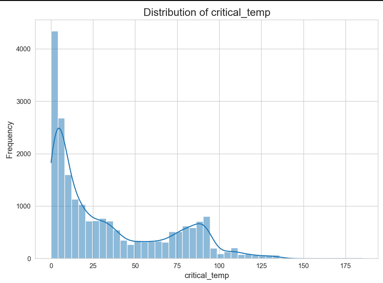
\includegraphics[scale=0.7]{t_c_distritbution.png}}
	\caption{$T_c$ distribution.}
	\label{TcDist}
\end{figure}

\begin{itemize}
	\item As visually displayed in ``Fig.~\ref{TcDist}'', the distribution exhibits a right-skewed (positive skew) shape, superficially resembling a Poisson distribution.
	\item However, the distribution is characterized by a high concentration of near-zero observations and a sharp peak, which deviates from a true Poisson process. Crucially, no negative values were observed, consistent with the physical nature of thermal conductivity.
	\item the trending line is the Kernel Density Estimate (KDE) showing the general density of the distribution.\\
\end{itemize}

Correlation analysis was performed on the derived chemical features to identify predictors strongly associated with the target variable.
\begin{figure}[htbp]
	\centerline{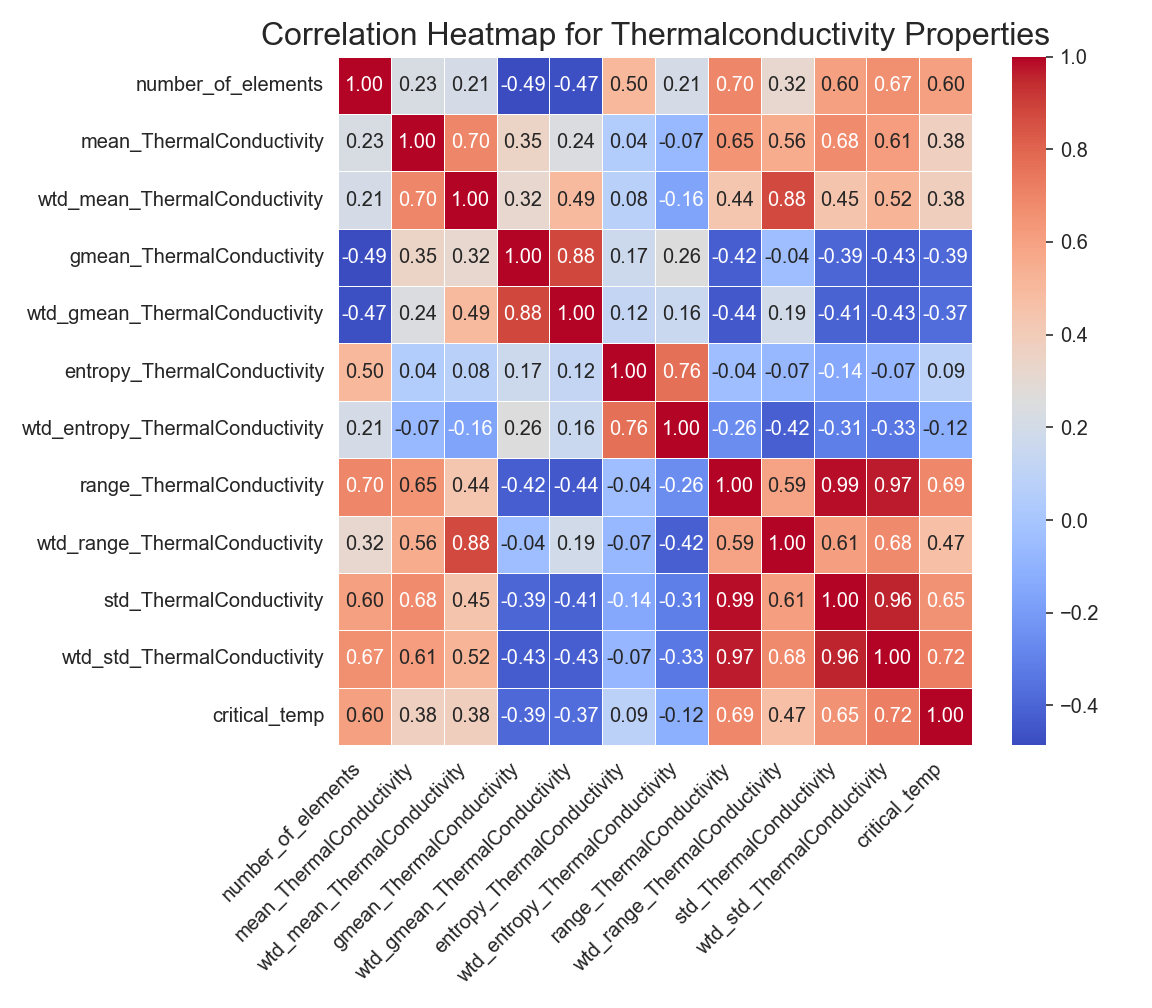
\includegraphics[scale=0.4]{ThermalConductivity_heatmap.png}}
	\caption{Thermal Conductivity Correlation within its own set.}
	\label{ThcCorr}
\end{figure}
\begin{itemize}
	\item Initially, multiple heatmaps, such as the example shown in ``Fig.~\ref{ThcCorr}'' for the Thermal Conductivity set, were generated to examine the correlation structure among various feature subsets, focusing on their linear relationship with $T_c$ and the feature \texttt{number\_of\_elements}.
\end{itemize}
\begin{table}[h]
	\centering
	\caption{Features Correlated with Critical Temperature}
	\label{WhlCorr}
	\begin{tabular}{|l|r|}
		\hline
		\textbf{Features} & \textbf{critical\_temp} \\
		\hline
		\texttt{critical\_temp} & 1 \\
		\texttt{wtd\_std\_ThermalConductivity} & 0.7212710792 \\
		\texttt{range\_ThermalConductivity} & 0.6876539119 \\
		\texttt{range\_atomic\_radius} & 0.6537590446 \\
		\texttt{std\_ThermalConductivity} & 0.6536319815 \\
		\texttt{wtd\_entropy\_atomic\_mass} & 0.6269304017 \\
		\texttt{wtd\_entropy\_atomic\_radius} & 0.6034939833 \\
		\texttt{number\_of\_elements} & 0.601068571 \\
		\texttt{range\_fie} & 0.6007903801 \\
		\texttt{wtd\_std\_atomic\_radius} & 0.5991986591 \\
		\texttt{entropy\_Valence} & 0.5985909069 \\
		\texttt{wtd\_entropy\_Valence} & 0.5896637026 \\
		\texttt{wtd\_std\_fie} & 0.5820132554 \\
		\texttt{entropy\_fie} & 0.5678169385 \\
		\texttt{wtd\_entropy\_FusionHeat} & 0.5632442681 \\
		\texttt{std\_atomic\_radius} & 0.559628574 \\
		\texttt{entropy\_atomic\_radius} & 0.5589374384 \\
		\texttt{entropy\_FusionHeat} & 0.5527087052 \\
		\texttt{entropy\_atomic\_mass} & 0.5436194092 \\
		\texttt{std\_fie} & 0.5418038102 \\
		\hline
	\end{tabular}
\end{table}
\begin{itemize}
	\item To consolidate this analysis and focus on the most influential predictors, a comprehensive correlation matrix was computed across the entire feature population. Feature selection was then performed by retaining only those features demonstrating a strong linear correlation with $T_c$.
	\item Specifically, only features with a Pearson correlation coefficient (r) greater than 0.53 were selected for model building. The final set of selected features is presented in ``Table~\ref{WhlCorr}''. This threshold ensured that only the features exhibiting the highest degree of linear association with $T_c$ were carried forward.\\
\end{itemize}



\subsubsection{\textbf{Model Fitting and Evaluation}}

In the process of model fitting and evaluation, the three different models were fitted against the \textbf{training set} and subsequently tuned by predicting on the \textbf{validation set}. The performance metrics for all models are summarized in a comparative table ``Table~\ref{model_comparison_basic}''.

\begin{table}[h]
	\centering
	\caption{Performance Metrics for Poisson, Tweedie, and MLR Models}
	\label{model_comparison_basic}
	\begin{tabular}{|l|c|c|c|}
		\hline
		\textbf{Metrics} & \textbf{Poisson} & \textbf{Tweedie} & \textbf{MLR} \\
		\hline
		Null Deviance    & 3750.86 & 8453.64 & 980.19 \\
		\hline
		Deviance         & 1131.13 & 2831.21 & 383.79 \\
		\hline
		AIC              & 15563.65 & -27070.60 & -14139.73 \\
		\hline
		BIC              & -153004.54 & -151304.46 & -15751.88 \\
		\hline
		Log-Likelihoods  & -7762.83 & 13554.30 & 7088.87 \\
		\hline
	\end{tabular}
\end{table}

Based on the statistical criteria, the \textbf{Tweedie GLM} emerged as the statistically preferred choice.
\begin{itemize}
	\item \textbf{Information Criteria (AIC and BIC)}: The Tweedie model exhibited the lowest (most negative) AIC and BIC values, indicating a superior balance between model fit and model complexity.
	\item \textbf{Log-Likelihood (logL)}: Consistent with the information criteria, the Tweedie model also demonstrated the highest logL, suggesting the better-fitting model. The substantial magnitude of the difference in AIC/BIC compared to the other models is noteworthy, implying a significantly better fit or effective regularization specific to the Tweedie distribution assumptions on this dataset.
\end{itemize}

While the Tweedie model was statistically favored, a closer look at the deviance revealed a minor conflict with the fit metrics:

\begin{itemize}
	\item \textbf{Deviance}: The Multiple Linear Regression (MLR) model achieved the lowest residual deviance (Deviance=383.79). Deviance, which measures the unexplained variation, suggests that the MLR model provided the best fit in terms of minimizing the error sum of squares relative to the null model.
	\item \textbf{Trade-off}: This discrepancy highlights the core difference between raw fit (Deviance) and penalized fit (AIC/BIC). Although the MLR model achieves the minimal residual deviation, the AIC and BIC values indicate that when the trade-off with the number of model parameters is considered, the \textbf{Tweedie model provides a statistically more robust and generalizable solution}.
\end{itemize}

\subsection{\textbf{Results}}
This section presents the final predictive performance of the selected models on the held-out \textbf{test set}, analyzes the diagnostic plots for the preferred model, and interprets the final coefficients and metrics.
\begin{figure}[htbp]
	\centerline{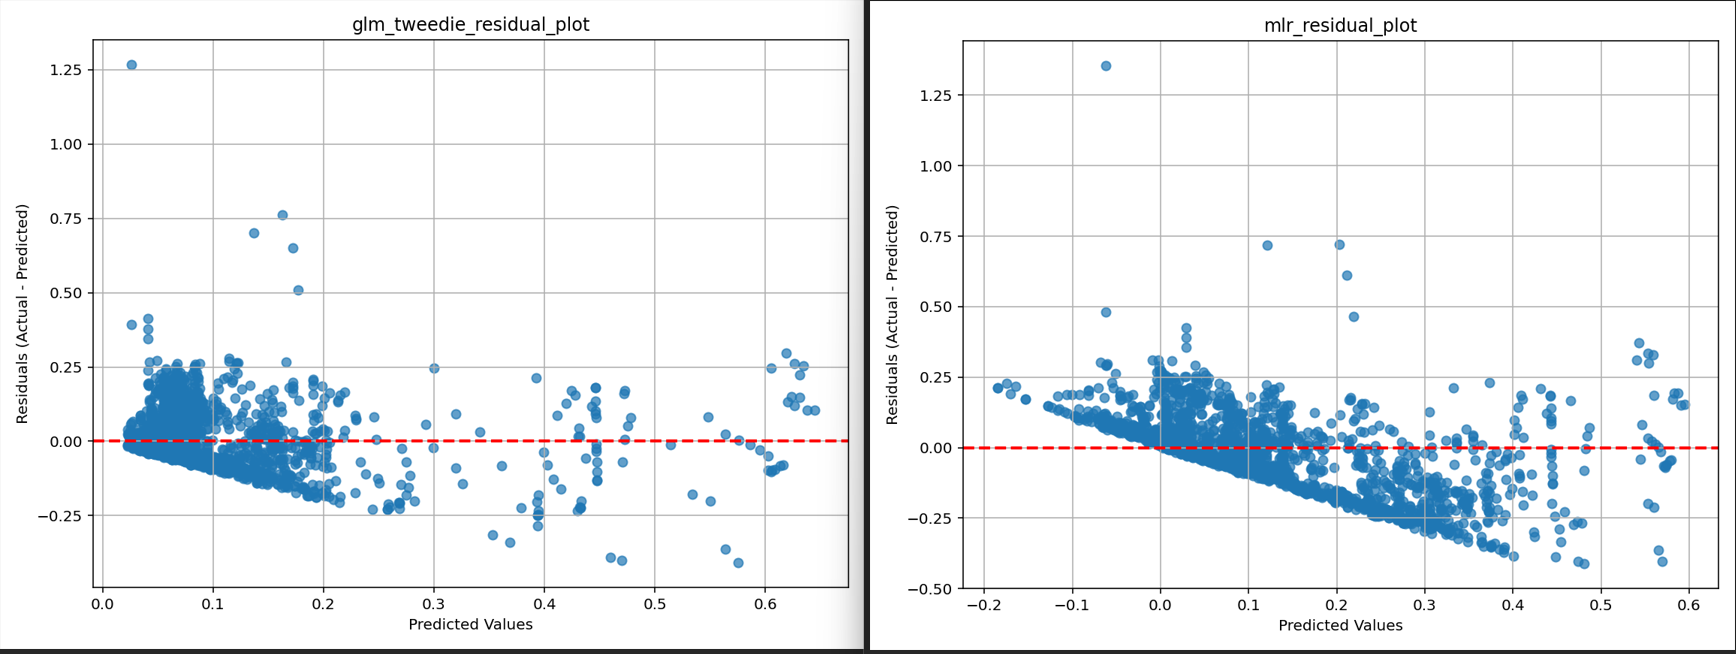
\includegraphics[scale=0.2]{residual_plots_mlr_vs_tweedie_test.png}}
	\caption{Residual Plots Tweedie GLM vs MLR Test Set}
	\label{test_residual_plot}
\end{figure}

The final predictive capabilities of the models were further examined through residual analysis, as illustrated in ``Fig.~\ref{test_residual_plot}''.
\begin{itemize}
	\item \textbf{Tweedie Model}: The residual plot for the Tweedie GLM model displays a distinct fanning-out pattern (heteroscedasticity). While this indicates the model's predictive variance increases with the magnitude of the predicted value, it is a common characteristic of models fit to count or positive, skewed data (like the target variable).
	\item \textbf{MLR Model}: The Multiple Linear Regression (MLR) model shows a clear negative trend in its residuals, which is to be expected as the distribution of Tc violates its assumptions.
	\item \textbf{Poisson GLM Model}: The Poisson GLM model, though not shown, has a similar and more compacted, fanning-out pattern compared to the Tweedie model.\\
\end{itemize}

\begin{table}[h!]
	\centering
	\caption{Tweedie GLM Model Regression Coefficients and Statistics}
	\footnotesize
	\label{tab:regression_results}
	\begin{tabular}{l r r r}
		\hline
		\textbf{Feature} & \textbf{Coef.} & \textbf{z} & \textbf{P$>|z|$} \\
		\hline
		number\_of\_elements & -0.463 & -2.348 & 0.019 \\
		wtd\_entropy\_atomic\_mass & 2.583 & 23.674 & 6.64975E-124 \\
		range\_fie & 5.726 & 18.253 & 1.96093E-74 \\
		wtd\_entropy\_atomic\_radius & -1.1479 & -7.507 & 6.00491E-14 \\
		range\_atomic\_radius & 1.699 & 9.153 & 5.55089E-20 \\
		wtd\_std\_atomic\_radius & 0.761 & 5.775 & 7.71026E-09 \\
		range\_ThermalConductivity & 1.005 & 4.727 & 2.269324E-06 \\
		std\_ThermalConductivity & -0.204 & -0.879 & 0.379 \\
		wtd\_std\_ThermalConductivity & 0.993 & 13.2758 & 3.20268E-40 \\
		entropy\_Valence & 2.713 & 8.888 & 6.19435E-19 \\
		wtd\_std\_fie & -1.499 & -12.1831 & 3.81256E-34 \\
		entropy\_fie & 1.985 & 2.002 & 0.045 \\
		wtd\_entropy\_FusionHeat & -0.157 & -1.922 & 0.0547 \\
		wtd\_std\_atomic\_radius & -1.357 & -5.959 & 2.53186E-09 \\
		entropy\_atomic\_radius & -2.371 & -2.517 & 0.012 \\
		entropy\_FusionHeat & 0.0686 & 0.601 & 0.5478 \\
		entropy\_atomic\_mass & -3.613 & -22.206 & 3.00824E-109 \\
		std\_fie & -4.019 & -13.407 & 5.48687E-41 \\
		\hline
	\end{tabular}
\end{table}

The final p-values associated with the Tweedie GLM model's coefficients provided a clear understanding of the features' statistical relevance:
\begin{itemize}
	\item \textbf{Statistically Significant Features}: The majority of the included features were confirmed to be \textbf{highly statistically significant} predictors of $T_c$ in the final model(i.e. p $\leq$ 0.05).
	\item \textbf{Insignificant Features}: The following features were found to be statistically insignificant, \texttt{std\_ThermalConductivity} and \texttt{entropy\_FusionHeat}. These features could be considered for \textbf{removal} in a future model refinement step to simplify the final structure without a significant loss in overall predictive power, thus further enhancing the model's interpretability.\\
\end{itemize}
\begin{table}[h!]
	\centering
	\caption{Models Regression Fit}
	\footnotesize
	\label{tab:regression_fit_results}
	\begin{tabular}{|l|c|c|c|}
		\hline
		\textbf{Metrics} & \textbf{Poisson} & \textbf{Tweedie} & \textbf{MLR} \\
		\hline
		MSE & 0.010422 & 0.010417 & 0.020016 \\
		\hline
		RMSE & 0.102087 & 0.102064 & 0.141478 \\
		\hline
		MAE & 0.071183 & 0.072239 & 0.106225 \\
		\hline
		MAPE & 269.64 & 302.48 & 447.73 \\
		\hline
	\end{tabular}
\end{table}

\indent The models were assessed on the unseen test set, and the predictive metrics remained largely consistent with the trends established during the validation stage. The Tweedie regression model continued to be the preferred choice.\\
\indent While the Tweedie model's performance metrics on the test set barely underperformed in comparison to the Poisson model (e.g., slightly higher RMSE), this marginal difference was observed on a significantly smaller test set.\\
\indent Given the Tweedie model's superior performance across the AIC and BIC—which indicated its overall robustness, better fit-to-complexity trade-off, and stability during the more extensive validation stage—we still selected the Tweedie model as the best GLM for the prediction of $T_c$.\\
\indent This decision prioritizes the model's proven stability and statistical rigor over a minor, potentially artifactual, difference on the smaller test subset.

\section{\textbf{Conclusion(s)}}

This study successfully investigated the relationship between derived material properties and the critical temperature $T_c$ of superconducting materials, aiming to determine if a statistically viable linear predictive model could be established.

The primary finding of this analysis is the development of a robust predictive framework for $T_c$ using a GLM.
\begin{itemize}
	\item \textbf{Optimal Model Selection}: The \textbf{Tweedie GLM} with a Compound Poisson-Gamma distribution was identified as the best predictive model. This choice was driven by the observation that the $T_c$ distribution exhibited characteristics closely aligned with the Poisson family, which the more flexible Tweedie distribution was able to accommodate better than a standard Poisson model.
	\item \textbf{Feature Simplification}: The feature set was significantly streamlined, reducing the number of predictive variables from 81 to 18 features, as detailed in ``Table~\ref{WhlCorr}''. This simplification maintains a high level of predictive power while substantially improving model simplicity.
	\item \textbf{Predictive Validation}: The low MSE achieved by the Tweedie GLM provides strong evidence that $T_c$ can be accurately predicted using a linear model based on a select, meaningful subset of the initial derived chemical features. The core focus of this work was validating the suitability of a linear model for this prediction task, which the results strongly support.\\
\end{itemize}

While the study confirmed a strong linear relationship, future research can build upon these findings:
\begin{itemize}
	\item \textbf{Model Complexity}: Explore non-linear models or more advanced Machine Learning algorithms (e.g. gradient boosting or neural networks) to potentially capture complex interactions and further improve predictive accuracy beyond the scope of a linear assumption.
	\item \textbf{Feature Refinement}: Conduct additional feature engineering by investigating potential methods to combine or transform the statistically insignificant features identified in the model. This could enhance the final feature set, reduce any residual redundancy, and potentially lead to a simpler, yet more powerful, predictive model.
	\item \textbf{Target Variable Transformation}: A key area for future investigation is exploring the effect of transforming the target variable $T_c$. Applying a mathematical transformation could potentially normalize the distribution, stabilize the variance, and further enhance the performance of a linear model.
\end{itemize}

\section*{\textbf{Appendix}}
	
\section*{Appendix A: Supplementary Materials and Software Usage}
\subsection*{Source Code Repository \label{app:code}}
The source code, data, and detailed implementation scripts for this project are available on GitHub (URL: https://github.com/gaguillen4384-dev/Data-Science/tree/main/DataMining\_1/Project\_1).

\subsection*{Software Usage Acknowledgment}
The text and documentation were edited and refined using Google Gemini.

\begin{thebibliography}{9} % '9' is for formatting the numbering (up to 9 items)
	
	\bibitem{hamidieh2018}
	Hamidieh, Kam. ``A data-driven statistical model for predicting the critical temperature of a superconductor.'' \textit{Computational Materials Science} 154 (2018): 346--354. DOI: 10.1016/j.commatsci.2018.07.052.
	
\end{thebibliography}

\vspace{12pt}

\end{document}
